\documentclass[main.tex]{subfiles}

\begin{document}

\section{From graphics pipeline to AI accelerator}
\begin{frame}
  \frametitle{Timeline}
  \begin{itemize}
    \item \textbf{1999---2003:} fixed-function graphics gives way to programmable
      vertex and pixel shaders.
    \item \textbf{2004:} Brook for GPUs demonstrates a high-level stream-programming
      model on top of graphics APIs.
    \item \textbf{2006---2007:} GeForce 8800 introduces a unified shader architecture;
      NVIDIA releases CUDA publicly in 2007.
    \item \textbf{2010:} Fermi adds a coherent cache hierarchy, ECC support, and much
      stronger support for C++ and scientific computing.
    \item \textbf{2017:} Volta introduces Tensor Cores for mixed-precision matrix
      multiply--accumulate.
    \item \textbf{2020---2024:} Ampere broadens Tensor Core formats; Hopper adds the
      FP8 Transformer Engine; Blackwell adds further low-precision and AI-specific hardware.
  \end{itemize}
\end{frame}

% TODO: continue polishing this.
\begin{frame}
  \frametitle{What shaped modern GPU architecture?}
  \only<1>{
    \begin{center}
      \textbf{New workloads cause generalization/programmability, established workloads cause specialization.}

      \vspace{0.7em}
      \begin{tikzpicture}[x=1.25cm,y=1cm,>=Latex,font=\scriptsize]
  \draw[very thick,-{Latex}] (0,0) -- (7.4,0);
  \foreach \x/\year/\label in {
    0/1999/{Fixed-function\\T\&L},
    1.4/2004/{Brook\\for GPUs},
    2.8/2006/{Unified\\shaders},
    4.2/2010/{Fermi\\compute},
    5.6/2017/{Tensor\\Cores},
    7/2022/{Transformer\\Engine}}
  {
    \draw[thick] (\x,0.12)--(\x,-0.12);
    \node[above=3pt,align=center] at (\x,0.12) {\label};
    \node[below=3pt] at (\x,-0.12) {\year};
  }
  \draw[blue!70!black,thick,-{Latex}] (0,1.05)--node[above]{more programmable}(4.2,1.05);
  \draw[orange!90!black,thick,-{Latex}] (4.2,1.05)--node[above]{AI specialization}(7,1.05);
\end{tikzpicture}

    \end{center}
  }

  \only<2>{
    \textbf{$<$2006: graphics first}
    \begin{itemize}
      \item GeForce 256 (1999) accelerated fixed-function transform and lighting.
      \item Later chips added programmable vertex and pixel shaders, but kept
        distinct stages and resources.
    \end{itemize}
    \centering

    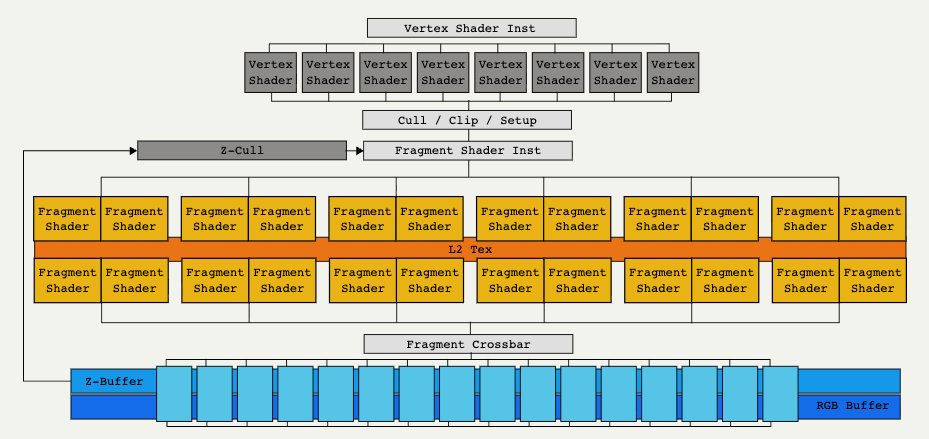
\includegraphics[width=.8\linewidth]{g71.png}

    {\tiny The G71 architecture (2005). Diagram source: Sanglard (2020).}
  }

  \only<3>{
    \textbf{2004: GPGPU before CUDA. Demand was always there.}
    \begin{itemize}
      \item Brook for GPUs compiled a stream language to graphics APIs.
      \item It showed useful non-graphics workloads could exploit GPU throughput,
        despite an awkward programming model.
    \end{itemize}
    \centering
    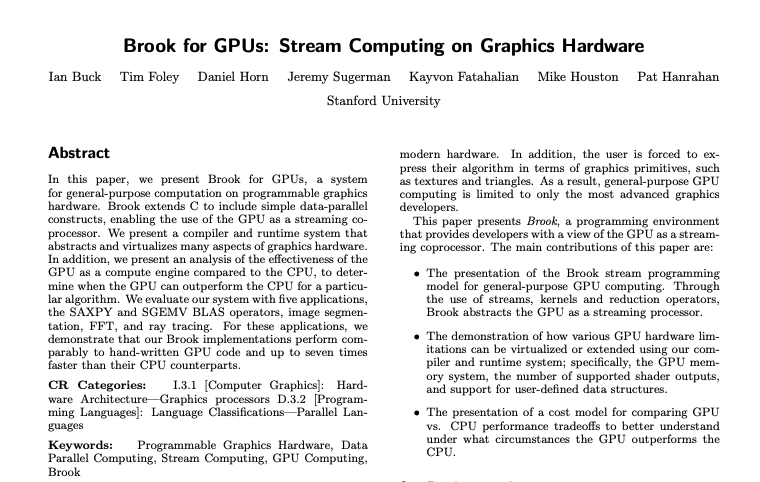
\includegraphics[width=\linewidth,height=.55\textheight,keepaspectratio]{brook-for-gpus.png}

    {\tiny Buck et al., ``Brook for GPUs,'' \emph{ACM TOG} 23(3), 2004.}
  }

  \only<4>{
    \textbf{2006-2007: increasing complexity necessitates unified compute}
    \begin{itemize}
      \item G80 ran vertex, geometry, and pixel work on unified pool of \textbf{Streaming Multiprocessors} (SM's).
      \item Publicly released in 2007, CUDA exposed this parallel machine
        without graphics API tricks.
    \end{itemize}
    \centering
    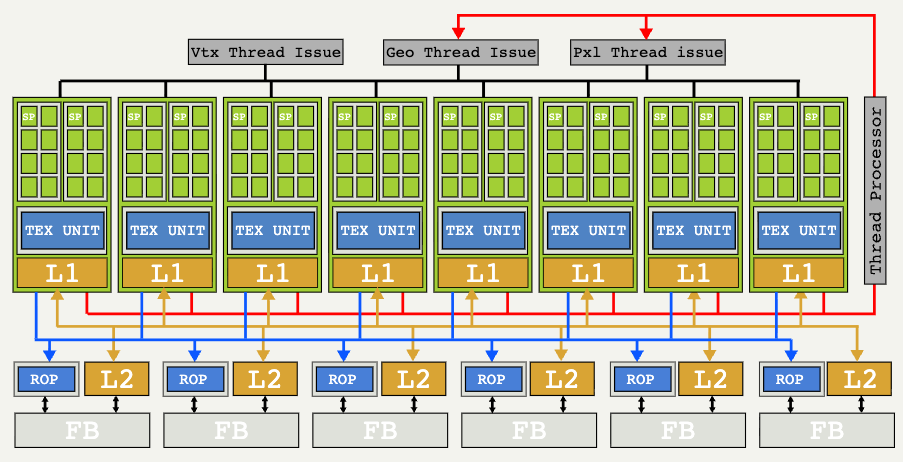
\includegraphics[width=\linewidth,height=.48\textheight,keepaspectratio]{g80.png}

    {\tiny G80 block diagram. Diagram source: Sanglard (2020); architecture described by Lindholm et al. (2008).}
  }

  % Fermi is not really that important for now.
  % \only<5>{
  %   \begin{columns}[T,onlytextwidth]
  %     \begin{column}{0.43\textwidth}
  %       \textbf{2010: Fermi makes compute first-class}
  %       \begin{itemize}
  %         \item Continues trend of general cores, scales horizontally.
  %         \item A unified L2 cache serves all SMs, establishes the heart of modern GPU memory hierarchy.
  %         \item Features for HPC like ECC and double precision FP.
  %       \end{itemize}
  %     \end{column}
  %     \begin{column}{0.55\textwidth}
  %       \centering
  %       \begin{tikzpicture}[font=\scriptsize,node distance=3mm]
  \foreach \x in {0,1.45,2.9} {
    \node[draw,fill=green!25,minimum width=1.25cm,minimum height=.75cm] (sm\x) at (\x,1.55) {SM};
    \node[draw,fill=purple!20,minimum width=1.25cm] at (\x,.93) {L1/shared};
  }
  \node[draw,fill=blue!20,minimum width=4.2cm,minimum height=.55cm] (l2) at (1.45,0) {unified L2 cache};
  \node[draw,fill=orange!25,minimum width=4.2cm,minimum height=.55cm] (dram) at (1.45,-.85) {Global Memory/DRAM};
  \foreach \x in {0,1.45,2.9} {\draw[-Latex] (\x,.67)--(\x,.3);}
  \draw[Latex-Latex] (l2)--(dram);
\end{tikzpicture}


  %       \vspace{0.5em}
  %       {\tiny Conceptual memory hierarchy. Based on NVIDIA, \emph{Fermi Compute Architecture Whitepaper}, 2009.}
  %     \end{column}
  %   \end{columns}
  % }
\end{frame}

\begin{frame}
  \frametitle{Takeaways}
  Our basic model of the GPU:
  \begin{itemize}
    \item SMs: primary compute unit
    \item CUDA Cores: like the "ALUs" of the SMs.
    \item L1 cache/Shared memory: cache for the SM
    \item Device/Global Memory: like RAM for a normal CPU system.
  \end{itemize}

  {\centering
    \resizebox{0.65\textwidth}{!}{\begin{tikzpicture}[font=\scriptsize,>=Latex]
  \foreach \x/\name in {0/sm0,3.2/sm1,6.4/sm2} {
    \node[
      draw,
      rounded corners,
      fill=green!12,
      minimum width=2.7cm,
      minimum height=2.05cm,
      label={[font=\bfseries]above:SM}
    ] (\name) at (\x,1.65) {};

    \foreach \dx/\dy in {-.65/.35,.15/.35,-.65/-.25,.15/-.25} {
      \node[draw,fill=green!30,minimum width=.55cm,minimum height=.42cm,font=\tiny]
        at ($(\name.center)+(\dx,\dy)$) {core};
    }
    \node[draw,fill=purple!20,minimum width=.85cm,minimum height=1.15cm,align=center]
      at ($(\name.center)+(.82,.05)$) {L1 /\\shared\\memory};
  }

  \node[draw,fill=orange!25,minimum width=9.1cm,minimum height=.65cm]
    (dram) at (3.2,-.15) {Device / Global Memory (DRAM)};

  \foreach \name in {sm0,sm1,sm2} {
    \draw[Latex-Latex] (\name.south) -- (\name.south |- dram.north);
  }
\end{tikzpicture}
}\par
  }

  \begin{block}{Whats next}
    How can we actually implement a matrix multiplication on a GPU? What tools
    and mental models do we need?
  \end{block}
\end{frame}

\end{document}
